\documentclass[tikz, border=10pt]{standalone}
\usepackage{iftex}
\ifluatex
  \usepackage{fontspec}
  \usepackage{unicode-math}
  \setmainfont{Fira Sans}
  \setmonofont{Fira Mono}
  \setmathfont{Fira Math}
  \setmathfont{STIX Two Math}[range={"29F5,"2216}]
\else
  \usepackage[T1]{fontenc}
\fi

\usepackage{amsmath}
\usepackage{tikz}
\usetikzlibrary{arrows.meta}
\tikzset{every node/.style={font=\Large}}

% Theme toggle: \darkbgfalse for light background preview.
\newif\ifdarkbg
\darkbgfalse
\ifdarkbg
  \colorlet{axiscol}{white}
  \colorlet{gridcol}{white!30!black}
  \colorlet{ticklabelcol}{white}
  \colorlet{funcol}{yellow!85!white}
  \colorlet{auxcol}{white!50!black}
\else
  \colorlet{axiscol}{black}
  \colorlet{gridcol}{black!25!white}
  \colorlet{ticklabelcol}{black}
  \colorlet{funcol}{blue!70!black}
  \colorlet{auxcol}{black!40!white}
\fi

% x: -1 to 7   (8 units)   xscale=0.85 → ~6.8 cm wide
% y: -3 to  5   (8 units)   yscale=0.85 → ~6.8 cm tall  (nearly square)
% Vertical asymptote at x = 0.
% Key point: (1, 2) — only clean integer point.
% Curve approaches -inf as x→0+, and f(7) ≈ 3.95 near top border.
\begin{document}
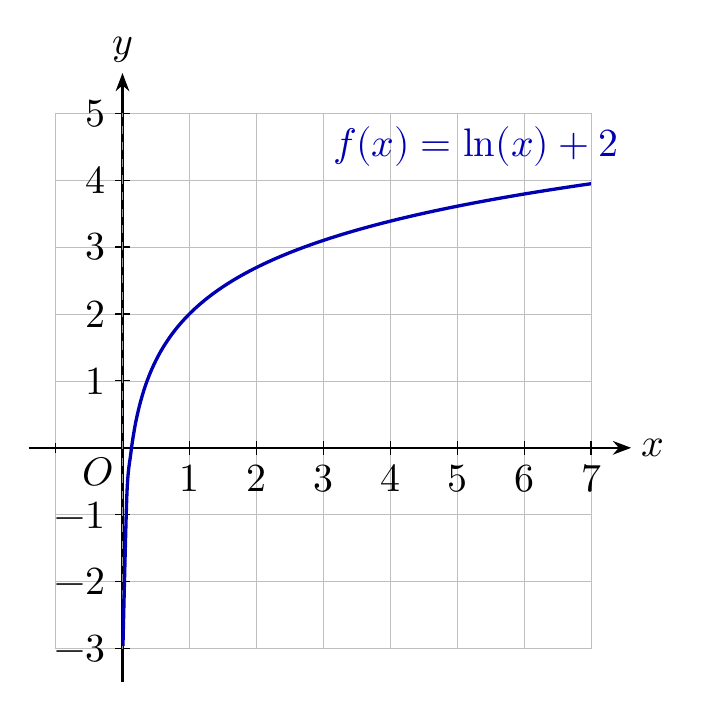
\begin{tikzpicture}[xscale=0.85, yscale=0.85, >=Stealth]

  % Cartesian grid.
  \draw[step=1, very thin, gridcol] (-1,-3) grid (7,5);

  % Axes.
  \draw[->, thick, axiscol] (-1.4,0) -- (7.6,0)
    node[right, text=axiscol] {$x$};
  \draw[->, thick, axiscol] (0,-3.5) -- (0,5.6)
    node[above, text=axiscol] {$y$};

  % Tick marks — x axis (only positive, function undefined for x≤0).
  \foreach \x in {1,2,3,4,5,6,7} {
    \draw[axiscol] (\x, 3pt) -- (\x, -3pt)
      node[below, text=ticklabelcol] {$\x$};
  }
  % Minor tick at x = -1 for scale context.
  \draw[axiscol] (-1, 2pt) -- (-1, -2pt);

  % Tick marks — y axis (labelled every 1).
  \foreach \y in {-3,-2,-1,1,2,3,4,5} {
    \draw[axiscol] (3pt,\y) -- (-3pt,\y)
      node[left, text=ticklabelcol] {$\y$};
  }

  % Origin label.
  \node[below left, text=axiscol] at (0,0) {$O$};

  % Vertical asymptote x = 0 (dashed).
  \draw[dashed, auxcol] (0,-3) -- (0,5);

  % Function curve: f(x) = ln(x) + 2, clipped to the window.
  \begin{scope}
    \clip (-1,-3) rectangle (7,5);
    \draw[domain=0.007:7, smooth, very thick, funcol, samples=120]
      plot (\x, {ln(\x) + 2});
  \end{scope}

  % Function label — upper-left, in the empty region left of the curve.
  \node[right, text=funcol] at (3,4.5) {$f(x)=\ln(x)+2$};

  % Key point (1, 2).
  % \node[circle, fill=funcol, inner sep=2pt] at (1,2) {};
  % \node[above right, text=funcol] at (1,2) {$(1,2)$};

\end{tikzpicture}
\end{document}
